\chapter{Hybrid Weak Galerkin - Continuous Galerkin Finite Element Method}
\label{chapter3}

In this chapter, we present a novel parallel computing method to effectively solve linear and nonlinear elasticity equations. The WG finite element method is newly developed by Dr. Junping Wang and Dr. Xiu Ye  \cite{wang2013weak}. We develop a novel hybrid element which combines the elements of both WG and CG finite element. The new hybrid element inherits the discontinuous feature of the WG method. To create a hybrid element, we treat the WG element as cargo ship and the CG element as the container. We insert multiple CG elements in one single WG element. 

The hybrid element takes advantages from both the WG and the CG element. For the WG element, it is discontinuous and can be calculated as a non-overlapping subdomain without extra unknown variables, such as Lagrangian multiplier. For the CG element, it's simple to construct and compute. The hybrid element use WG element as the subdomain boundary interface and CG and interior refine elements.

Like the standard FEM, the WG method can be used to solve generic partial differential equations. An advanced feature of the WG finite element method is that the entire problem can be decomposed into multiple local problems. In these local problems, the differential operators are approximated and reconstructed by small-size matrices. The WG method provides optimal orders of accuracy in spatial discretization for difficult problems on serial computers. However, the performance of the WG method on parallel computers has not yet been examined.

This chapter is organized as following. We first introduce the weak Galerkin method and the derivations of the bilinear form of nonlinear elasticity equation. Then we discuss the details of matrix construction. An improved stabilizer is designed for implementing time marching schemes. For the numerical method, we present the details of the parallel scheme including the explicit Central Difference method and the implicit time marching scheme, the Newmark-Beta method \cite{adeli1978algorithms}. At the end of this chapter, we present the numerical results of one-dimensional linear and nonlinear elastic equation. The second order accuracy are achieved with observed superlinear speedup.

\section{Nonlinear Elasticity Equation}

Consider an elastic body subject to an exterior force $ \mathbf{f} $, we denote the computational domain as $ \Omega $ and its continuous boundary as $ \Gamma = \partial \Omega $. The governing equation for elasticity can be written as
\begin{equation}
-\nabla \cdot \boldsymbol{\sigma(u)} = \mathbf{f}, \quad in \quad \Omega
\end{equation}
\begin{equation}
\mathbf{u} = \hat{\mathbf{u}},  \qquad on \quad \Gamma
\end{equation}
where $ \boldsymbol{\sigma(u)} $ is Cauchy stress. For isotropic and homogeneous materials, the stress-strain relation is
\begin{equation}
\boldsymbol{\sigma(u)} = 2\mu \varepsilon(\mathbf{u}) + \lambda (\nabla \cdot \mathbf{u}) \mathbf{I}
\end{equation}
the $ \mu $ and $ \lambda $ are Lame indices which can be written as
\begin{equation}
\lambda = \frac{E\nu}{(1 + \nu)(1 - 2\nu)}
\end{equation}
where $ E $ is the elasticity modulus and $ \nu $ is Poisson's ratio. 

The geometric nonlinear strain-displacement relation can be written as following format
\begin{equation}
\boldsymbol{\varepsilon(u)}= \frac{1}{2} (\nabla u + \nabla u^{T} - (\nabla u^{T}) \cdot \nabla u)
\end{equation}

The weak function on domain is $ u = \{u_0, u_b\} $, $ u_{0} \in L^{2} (T)$. The first function $ u_0 $ represents the interior domain of the function $ u $. The second function $ u_{b} $ represents the boundary value of function $ u $. The key notion is that for two functions $ u_0 $ and $ u_{b} $ are independent with each other. The weak function is defined as 
\begin{equation}
U_{h} = \{ u = \{u_{0}, u_{b} \}: u_{0} \in P_{j} (T^{0}), u_{b} \in P_{l} (e), e \subset \partial T \}
\end{equation}

The key of the weak Galerkin method is to approximate the solution in weak discrete space $ S(T) $. The discrete weak gradient $ \nabla_{w} u \in [P_{r} (T)]^{d} $ for $ u \in V_{h} $ on each element $ T $:

\begin{equation}
(\nabla_{w}, q)_{T} = -(u_{0}, \nabla \cdot q)_{T} + \langle u_{b}, q \cdot \mathbf{n} \rangle_{\partial T}
\end{equation}

for the discrete weak divergence, $ \nabla_{w} \cdot \mathbf{u} in [P_{r} (T)]^{d} $ is defined 
\begin{equation}
(\nabla_w \cdot u, q)_{T} = -(u_{0}, \nabla q)_{T} + \langle u_{b} \cdot \mathbf{n}, q \rangle_{\partial T}
\end{equation}

Then we can define the weak linear strain tensor by using the weak gradient
\begin{equation}
\varepsilon_{w} (u) = \frac{1}{2} (\nabla_{w} u + \nabla_{w} u^{T})
\end{equation}

Analogously, the nonlinear weak strain tensor is defined by 
\begin{equation}
\varepsilon_{w} (u) = \frac{1}{2} (\nabla_{w} u + \nabla_{w} u^{T} + (\nabla_w u^{T}) \cdot \nabla_w u ) 
\end{equation}

The weak stress can be defined as
\begin{equation}
\sigma_{w} (u) = 2 \mu \epsilon_{w}(u) + \lambda(\nabla_{w} \cdot u) \mathbf{I}
\end{equation}

The weak form of governing equation of continuous Galerkin method as
\begin{equation}
a(\mathbf{u}, \mathbf{v}) = (\mathbf{f}, \mathbf{v})
\end{equation}
the above approximation function $ v $ and the gradient $ \nabla v $ is not well defined for the discontinuous feature of weak Galerkin method. The new form is 
\begin{equation}
a(\mathbf{u}_{w}, \mathbf{v}_{w}) + s(\mathbf{u}, \mathbf{v}) = (\mathbf{f}, \mathbf{v})
\end{equation}
the term $ s(\mathbf{u}, \mathbf{v}) $ is a stabilizer enforcing a weak continuity which measures the discontinuity of the finite element solution. The governing equation in weak form can be introduced by two bilinear equations
\begin{equation}
s(\mathbf{u}, \mathbf{v}) = \sum_{T\in \Omega}^{N} h_{T}^{-1} \langle Q_{b} u_{0} - u_{b}, Q_{b} v_{0} - b_{b} \rangle_{\partial T}
\end{equation}
where $ Q_{b} $ is the projection parameter defined by the interior and boundary value. $ h_{T} $ is the characteristic length of mesh element. It is a constant number which usually is taken as 1.

The governing equation has the weak form as
\begin{equation}
a(\mathbf{u}_{w}, \mathbf{v}_{w}) = \sum_{T \in \Omega}^{N} 2(\mu \varepsilon_w (u), \varepsilon_{w} (v))_{T} + \lambda(\nabla_{w} \cdot \mathbf{u}, \nabla_{w} \cdot \mathbf{v})_{T}
\end{equation}

\section{Hybrid WG-CG Element}

In this section, we introduce the design of hybrid element, the construction of the basis functions. The one dimensional WG element has the shape function
\begin{equation}
\phi_{0}^{1} = \frac{x - x_{i +1}}{x_{i} - x_{i +1}}, \quad \phi_{b}^{1} = 1
\end{equation}

\begin{equation}
\phi_{0}^{2} = \frac{x - x_{i}}{x_{i + 1} - x_{i}}, \quad \phi_{b}^{2} = 1
\end{equation}

\begin{figure}[H]
	\centering
	\begin{tabular}{c}
		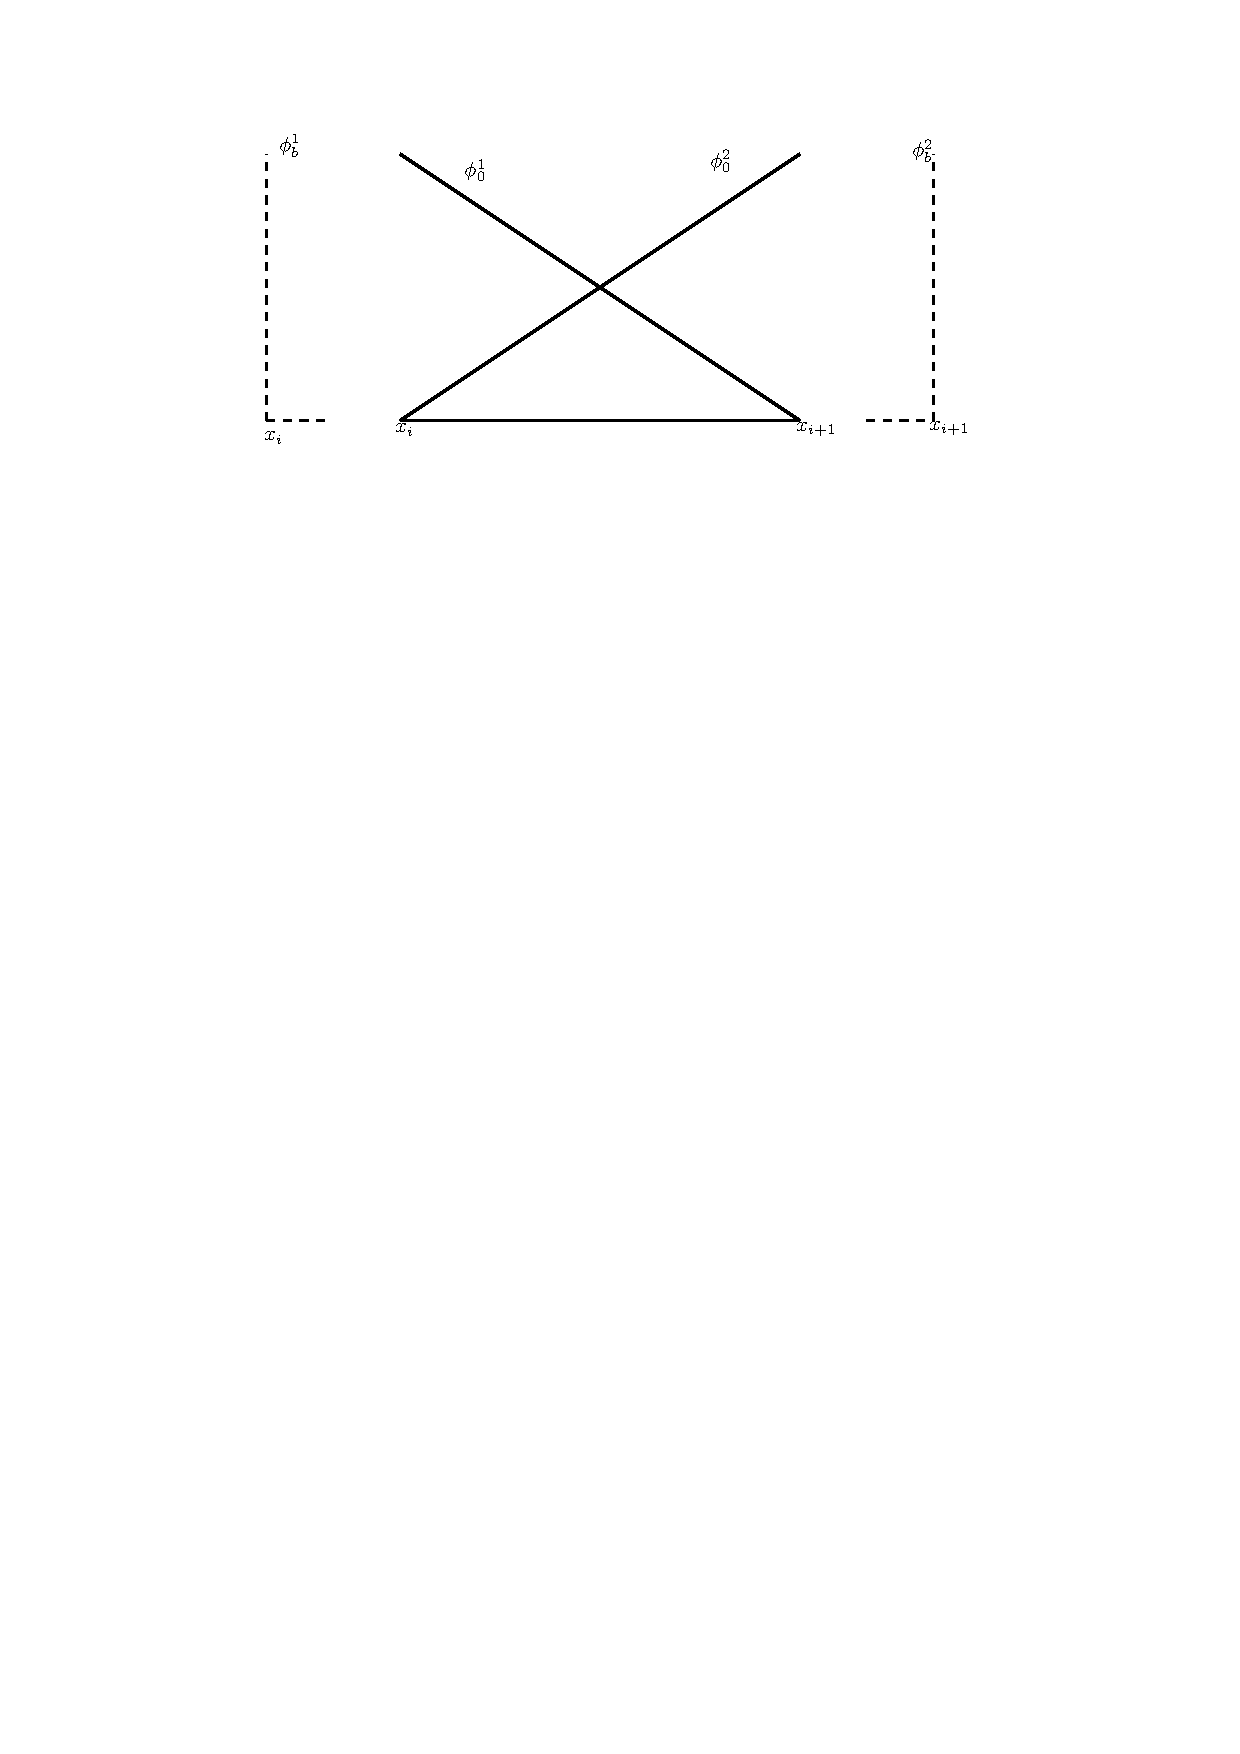
\includegraphics[width=0.7\textwidth]{./pics/oneD}
	\end{tabular}
	\caption{\footnotesize Basis function of one dimensional weak Galerkin element}
\end{figure}

Based on the weak gradient function, the boundary basis functions are independent of the interior basis functions, Therefore, we can insert an arbitrary number of CG element basis functions into the WG element. Each weak Galerkin element is considered as one sub-element that neighbored with adjacent elements. The interior CG elements are corrected by the coarse mesh which is the WG element. The boundary basis function of WG element is shared by adjacent elements and constitute the coarse mesh. The newly designed basis function of hybrid element can be illustrated as

\begin{figure}[h]
	\centering
	\begin{tabular}{c}
		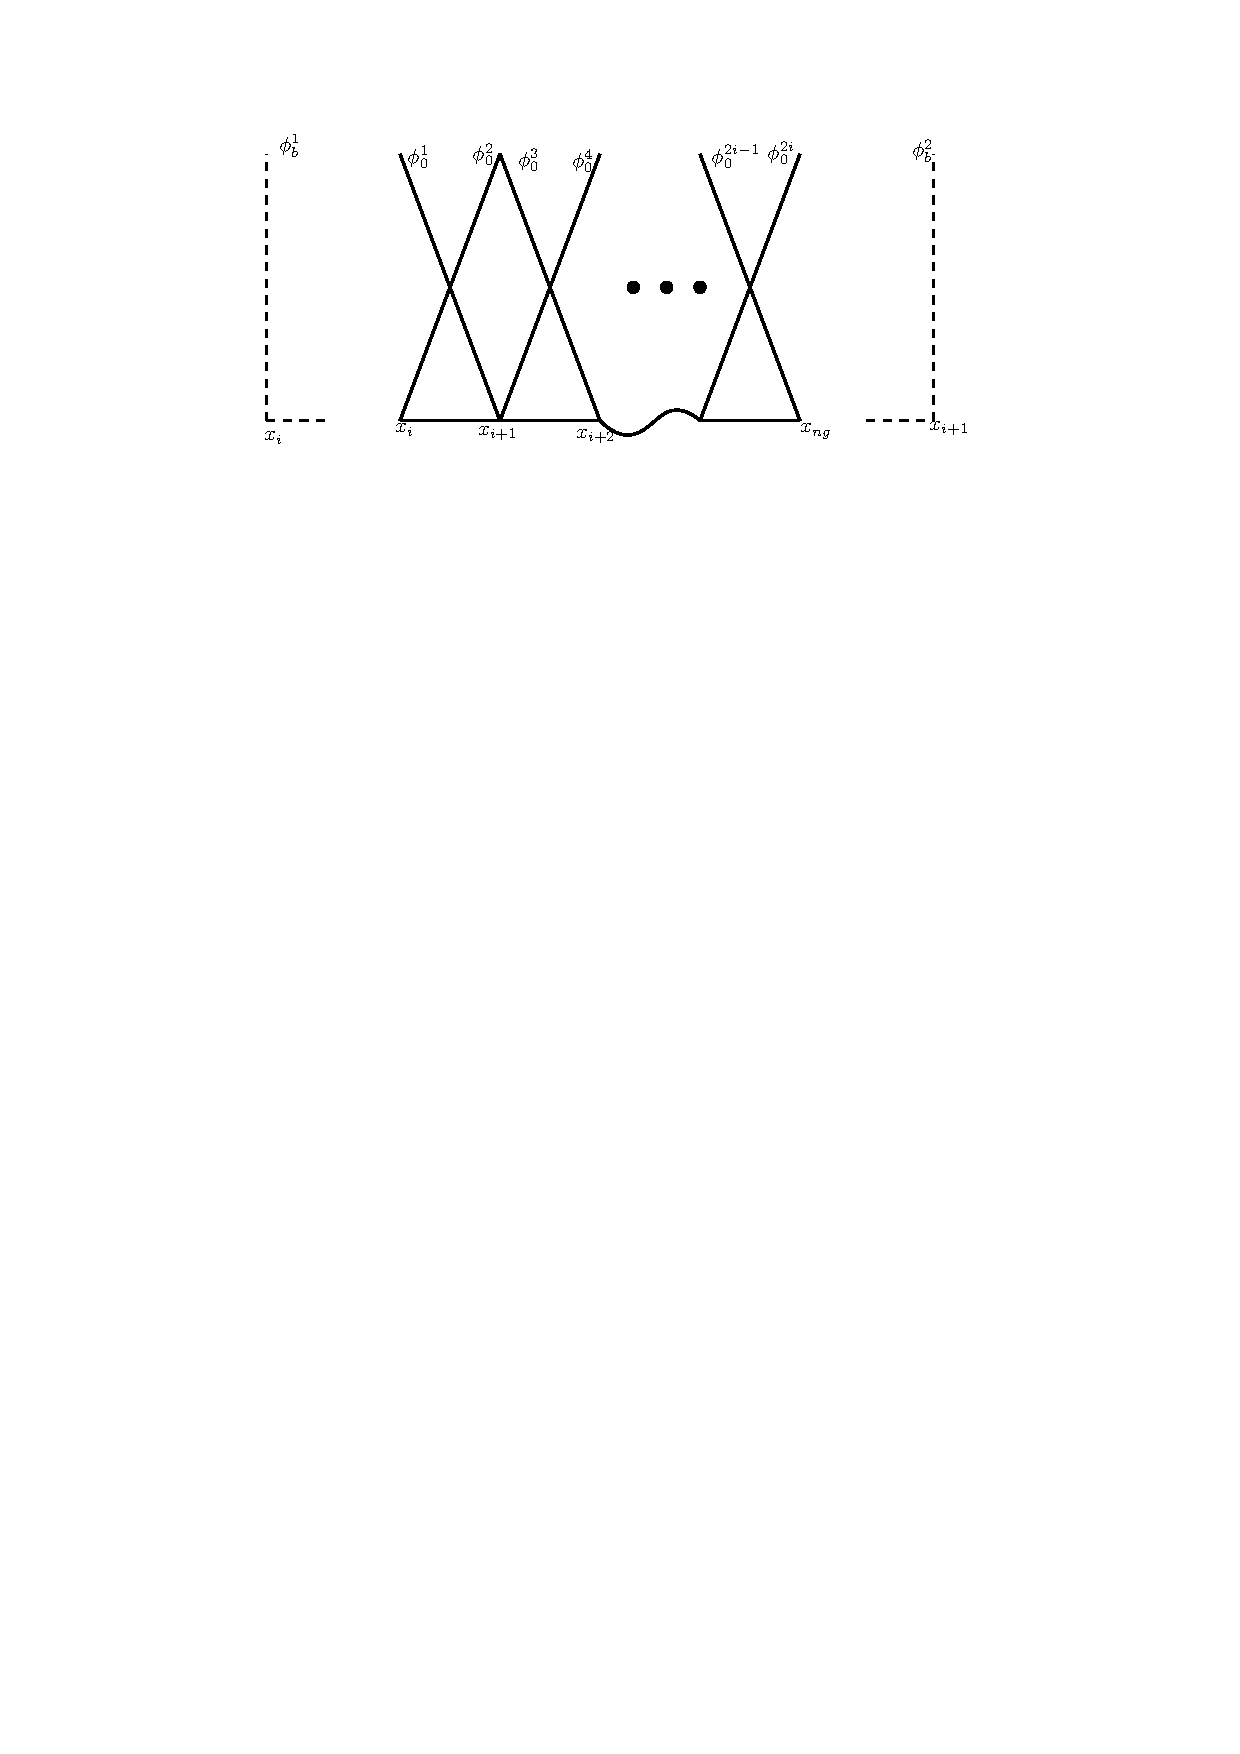
\includegraphics[width=0.7\textwidth]{./pics/hybrid}
	\end{tabular}
	\caption{\footnotesize Basis function of hybrid WG-CG element, an arbitrary number of CG elements are inserted into WG element}
\end{figure}

As above figure, in one WG element, there are multiple CG element basis functions. All the interior basis functions are linear and shared the same boundary basis functions of WG element. This is the illustration of the hybrid element basis functions.

\section{The Improved Stabilizer}

\subsection{Deficiency of Original Stabilizer}

Here we present the parallel computing scheme for one dimensional linear and nonlinear elastic equations. The governing equation for dynamic equation is 
\begin{equation}
M\ddot{u} + Ku = f
\end{equation}

In the hybrid elements, the information of mass is missing for the corresponding boundary values. The original governing equation in matrix form is
\begin{equation} \label{eq:incomp}
\begin{bmatrix}
M_{00} & 0 \\0 & 0 \\
\end{bmatrix}\begin{bmatrix}
\ddot{u}_{0} \\ \ddot{u}_{b} \\
\end{bmatrix} + \begin{bmatrix}
K_{00} & K_{0b} \\ K_{b0} & K_{bb} \\
\end{bmatrix} \begin{bmatrix}
u_{0} \\ u_{b} \\
\end{bmatrix} = \begin{bmatrix}
f_{0} \\ 0 \\
\end{bmatrix}
\end{equation}

from above equation we can find that the mass matrix for $ \ddot{u}_{b} $ is not complete. The information of mass is missing on the boundary basis functions. Under this circumstance, the explicit time marching scheme is unable to initiate. 


\subsection{Improvement}
To avoid the deficit of time marching scheme, we introduce a newly designed stabilizer, namely, the generic stabilizer.
\begin{equation}
s(\mathbf{u}, \mathbf{v}) = \sum_{T \in \Omega}^{N} h_{T}^{-1} \langle Q_{b} \ddot{u}_{0} - \ddot{u}_{b}, Q_{b} v_{0} - v_{b} \rangle_{\partial T}
\end{equation}

Consider the Central difference method as 
\begin{equation} \label{eq:cd}
\frac{\partial^{2} u}{\partial^{2} t} = \frac{u^{n + 1} - 2 u ^{n} + u^{n - 1}}{(\Delta t)^{2}}
\end{equation}

For one stabilizer matrix $ h^{-1} \langle Q_{b} \ddot{u} - \ddot{u}_{b}, Q_{b} v_{0} - v_{b} \rangle $, we apply Eq. \eqref{eq:cd} on it and rewrite it as
\begin{equation}
\langle  h^{-1} \frac{Q_{b} (u^{n + 1}_{0} - 2 u ^{n}_{0} + u_{0}^{n - 1})}{(\Delta t)^{2}}, Q_{b} v_{0} - v_{b} \rangle - h^{-1} \langle \frac{u_{b}^{n + 1} - 2u_{b}^{n} + u_{b}^{n - 1}}{(\Delta t)^{2}} , Q_{b} v_{0} - v_{b} \rangle
\end{equation}

Then we calculate the boundary integral and write the result in matrix form $ S $. The stabilizer is written in
\begin{equation}
\frac{h^{-1}}{(\Delta t)^{2}} \langle Q_{b} u_{0}^{n + 1} - u_{b}^{n + 1} , Q_{b} v_{0}- v_{b} \rangle - \frac{2h^{-1}}{(\Delta t)^{2}} \langle Q_{b} u_{0}^{n} - u_{b}^{n} , Q_{b} v_{0}- v_{b} \rangle + \frac{h^{-1}}{(\Delta t)^{2}} \langle Q_{b} u_{0}^{n - 1} - u_{b}^{n - 1} , Q_{b} v_{0}- v_{b} \rangle 
\end{equation}


\begin{equation}
\frac{h^{-1}}{(\Delta t)^{2}} \begin{pmatrix}
\begin{bmatrix}
S_{00} & S_{0b} \\ S_{b0} & S_{bb} 
\end{bmatrix} \cdot 
\begin{bmatrix}
u_{0}^{n + 1} \\ u_{b}^{n + 1}
\end{bmatrix}
 - 2\begin{bmatrix}
S_{00} & S_{0b} \\ S_{b0} & S_{bb}
\end{bmatrix} \cdot
\begin{bmatrix}
u_{0}^{n} \\ u_{b}^{n}
\end{bmatrix} + 
\begin{bmatrix}
S_{00} & S_{0b} \\ S_{b0} & S_{bb} 
\end{bmatrix} \cdot
\begin{bmatrix}
u_{0}^{n - 1} \\ u_{b}^{n - 1}
\end{bmatrix}
\end{pmatrix}
\end{equation}

We combine the discretized stabilizer with the incomplete equation Eq. \eqref{eq:incomp}, we can construct the governing equation in a new matrix form
\begin{eqnarray} \label{eq:newForm}
&& h^{-1}\begin{bmatrix}
M_{00} + S_{00} & S_{0b} \\ S_{b0} & S_{bb}
\end{bmatrix} \cdot \begin{bmatrix}
u_{0}^{n + 1} \\ u_{b}^{n + 1}
\end{bmatrix} + (\Delta t)^{2} 
\begin{bmatrix}
K_{00} & K_{0b} \\ K_{b0} & K_{bb}
\end{bmatrix} \cdot \begin{bmatrix}
u_{0}^{n + 1} \\ u_{b}^{n + 1}
\end{bmatrix}\\
& =& 2 h^{-1} \begin{bmatrix}
S_{00} & S_{0b} \\ S_{b0} & S_{bb}
\end{bmatrix} \cdot
\begin{bmatrix}
u_{0}^{n} \\ u_{b}^{n}
\end{bmatrix} - h^{-1}\begin{bmatrix}
S_{00} & S_{0b} \\ S_{b0} & S_{bb}
\end{bmatrix} \cdot
\begin{bmatrix}
u_{0}^{n - 1} \\ u_{b}^{n - 1}
\end{bmatrix} + (\Delta t)^{2} \begin{bmatrix}
f_{0} \\ 0
\end{bmatrix}
\end{eqnarray}

In Eq. \eqref{eq:newForm}, the mass matrix has completed with $ M_{bb} = S_{bb} $ information for boundary unknown variables. In the time marching scheme, the $ M_{bb}^{-1} $ produces valid result.

The original stabilizer requires that the values in the equation must be the same category. We extend the rule to all the unknown variables in the bilinear form. After the injection of the new stabilizer, the above equation becomes

\begin{equation}
\begin{bmatrix}
M_{00} & 0 \\ 0 & M_{bb}
\end{bmatrix}\begin{bmatrix}
\ddot{u}_{0} \\ \ddot{u}_{b}
\end{bmatrix} + \begin{bmatrix}
K_{00} & K_{0b} \\
K_{b0} & K_{bb} 
\end{bmatrix} \begin{bmatrix}
u_{0} \\ u_{b}
\end{bmatrix} = \begin{bmatrix}
f_{0} \\ 0
\end{bmatrix}
\end{equation}

Consequently, both explicit and implicit time marching scheme can be implemented on above matrices.

\subsection{Parallel Computing Method}

For both linear and nonlinear equations, we implement the implicit time marching scheme, the Newmark-Beta method. It has the following steps

\begin{equation}
\ddot{u}_{0}^{n+1} = \frac{(u_{0}^{n+1} - \tilde{u}_{0})}{\beta \Delta t^{2}}
\end{equation}
\begin{equation}
\ddot{u}_{b}^{n+1} = \frac{(u_{b}^{n+1} - \tilde{u}_{b})}{\beta \Delta t^{2}}
\end{equation}

The $ \tilde{u} $ represents the intermediate step, then we can use it to calculate the value of next step

\begin{equation}
\tilde{u}_{0} = u_{0}^{n} + \dot{u}_{0}^{n} \Delta t + \frac{1}{2} \Delta t^{2} \ddot{u}_{0}^{n} (1 - 2 \beta)
\end{equation}

\begin{equation}
\tilde{u}_{b} = u_{b}^{n} + \dot{u}_{b}^{n} \Delta t + \frac{1}{2} \Delta t^{2} \ddot{u}_{b}^{n} (1 - 2 \beta)
\end{equation}

To reduce the local unknown variable $ u_{0} $ into a smaller size global matrix of unknown variable $ u_{b} $, we apply the Schur complement method. The correlation between interior unknown variables and boundary variables is following equation

\begin{equation}
u_{0}^{n+1} = -K_{00}^{-1} K_{0b} u_{b}^{n+1} + K_{00}^{-1} g_{1}
\end{equation}

Therefore, the original large sparse global matrix is transformed into a small condensed global matrix with the only one set of unknown variables, $ u_{b} $. The governing equation has the new form
\begin{equation}
u_{b}^{n+1} = [K_{b0}(-K_{00}^{-1}K_{0b}) + K_{bb}]^{-1} (g_{2} - K_{b0} (K_{00}^{-1} g_{1}))
\end{equation}

Then we can simplify the above equation into
\begin{equation}
u_{b}^{n+1} = K^{'} f^{'}
\end{equation}

From above equations, the boundary unknown variable $ u_{b} $ is updated. In each time step, we convert local unknown variable $ u_{0} $ to $ u_{b} $ through local Schur complement method to reduce the computational cost. After condensing the matrix, we can calculate the solution by matrix inversion. 

\subsection{The Parallel Computing Work Flow}

For one-dimensional elastic equation, the original governing equation can be converted to a sparse tri-diagonal stiffness matrix to a blocked decomposed submatrices

 \begin{figure}[H]
 	\centering
 	\begin{tabular}{c}
 		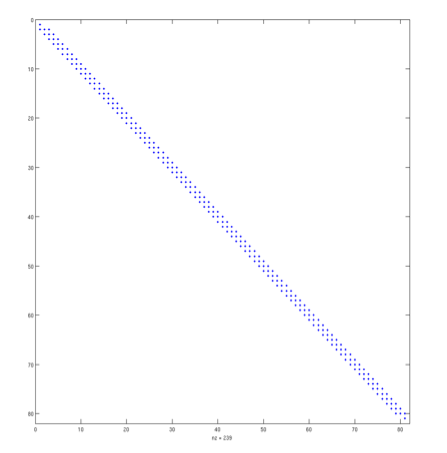
\includegraphics[width=0.5\textwidth]{./pics/matrix1.png}
 	\end{tabular}
 	\caption{\footnotesize Global sparse tri-diagonal stiffness matrix}
 \end{figure}
 
 For the WG element, the global matrix is constructed as above figure. The elements are continuously arranged. The parallel computing scheme such as Schur complement method cannot be directly applied. An external loading vector like Lagrangian multiplier is required. Our hybrid WG-CG element method is discontinuous, it will provide a discontinuous matrix form as below figure. 
 
  \begin{figure}[H]
  	\centering
  	\begin{tabular}{c}
  		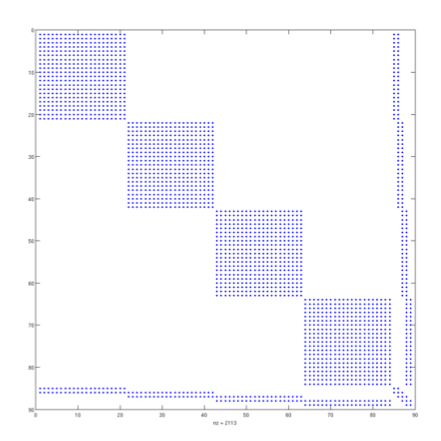
\includegraphics[width=0.5\textwidth]{./pics/hmatrix1.png}
  	\end{tabular}
  	\caption{\footnotesize Blocked stiffness matrix after domain decomposition}
  \end{figure}
  
  The original large sparse stiffness matrix is compressed in a very small matrix on the right bottom corner by using Schur complement method. In another word, the main computational load is split into the calculation of square matrices. Each square matrix represents the interior unknown variables in one single hybrid element. The size of hybrid element is determined by the number of interior CG elements since the boundary basis function remains the same. The entire computational domain is decomposed into multiple subdomains and each subdomain corresponds to one single processor. After the global calculation, the interior unknown variables can be recovered through local computing.
  
  The parallel computing work flow chart is described as following
  
    \begin{figure}[h]
    	\centering
    	\begin{tabular}{c}
    		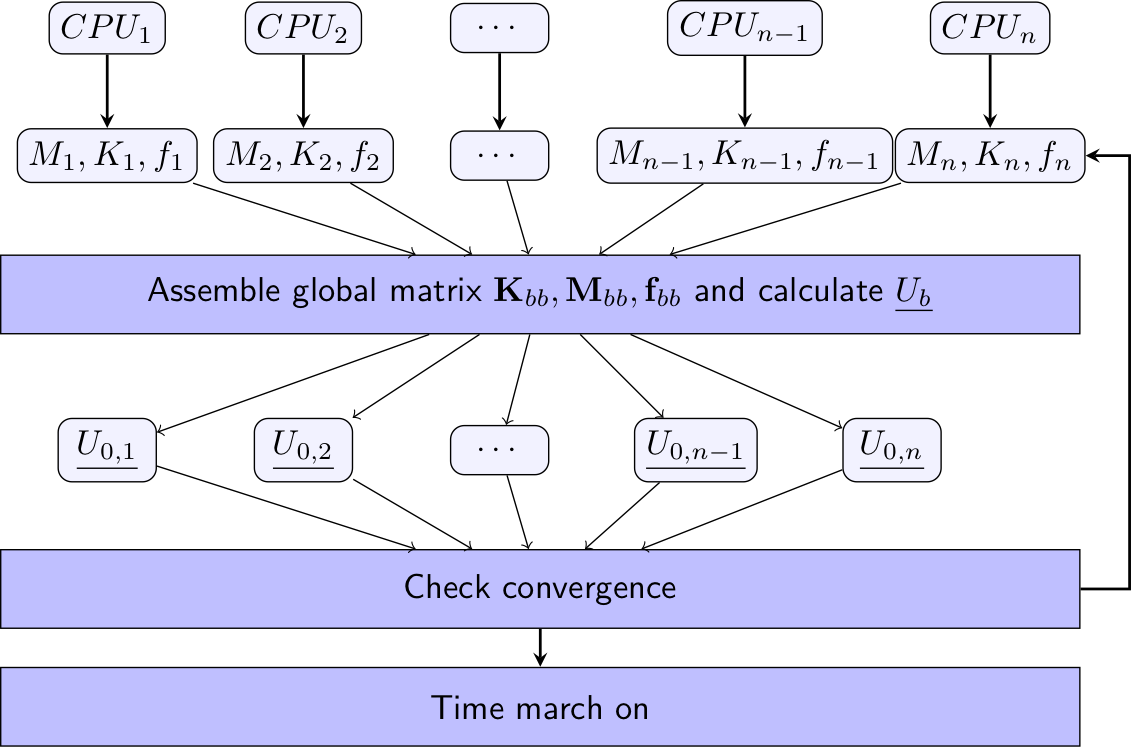
\includegraphics[width=0.6\textwidth]{./pics/flowchart1.png}
    	\end{tabular}
    	\caption{\footnotesize Parallel computing workflow chart for WG-CG method}
    \end{figure}
    
   \begin{enumerate}
   	\item Each CPU reads in preprocessed file and initiates MPI communication\cite{gropp1996high}.
   	\item Every hybrid element is dealt by each individual processor. Local stiffness matrices and load vectors are constructed on parallel machine.
   	\item The global stiffness boundary matrix is assembled additively. The global boundary unknown variables are obtained and passed to each processor through MPI communication.
   	\item Once the global residual is less than the tolerant value, current Newmark-Beta time iteration complete and move to the next time step.
   \end{enumerate}
   
   To accelerate the performance, we use the open source library such as LAPACK/BLAS to calculate the computationally expensive operators in terms of the block Cholesky elimination, matrix multiplication and vector operations. This implementation largely benefits the programming process and works very well among different high performance computing platforms.
   
   The software has been tested on the George Washington University super computing cluster, ColonialOne, with Xeon E5-2650v2 2.6GHz 8-core processors with 128 GB of RAM each.
   
   \section{Numerical Results}
   
   \subsection{Geometric linear elastic equation}
   
   We design a numerical test to verify the hybrid element with analytical solution $ u = sin (2 \pi x) $. In each WG element, we set 20 CG elements and then observe the accuracy of $ u_0 $, $ u_b $ and the effect of stabilizer.
   
      \begin{figure}[H]
      	\centering
      	\begin{tabular}{c}
      		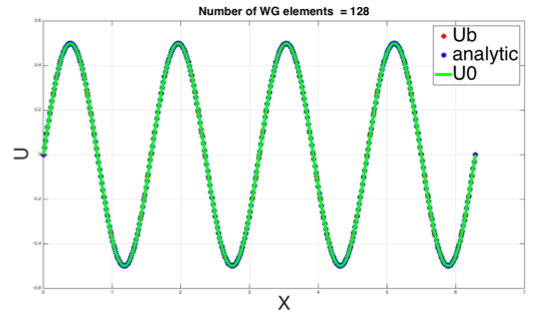
\includegraphics[width=0.8\textwidth]{./pics/result1d1.png}
      	\end{tabular}
      	\caption{\footnotesize Linear elastic equation results for hybrid WG-CG element}
      \end{figure}
      
      \begin{table}[h]
      	\setlength{\tabcolsep}{2pt} {
      		\caption{ Error and accuracy of hybrid WG-CG element for linear elasticity.}
      		\label{Tab:hwgcg l1}
      		\vspace{-5pt}
      		\begin{center}
      			%	\scalebox{0.6}{
      			\begin{tabular}{c|c|c|c|c}
      				\hline
      				\multicolumn{5}{c}{\# CG = 20} \\
      				\hline
      				\#WG & $ E (u_{0}) $ & $ O(u_{0}) $ & $ E(u_{b})  $& $ O(u_{b})  $\\
      				\hline
      				$ 16 $ & $ 1.7636e-4 $ & - & $ 3.8909e-4 $ & - \\
      				\hline
      				$ 32 $ & $ 4.4745e-5 $ & $ 1.98 $& $ 9.8515e-5 $ & $ 1.99 $ \\
      				\hline
      				$ 64 $ & $ 1.1271e-5 $ & $ 1.99 $ & $ 2.4744e-5 $ & $ 1.99 $ \\
      				\hline
      				$ 128 $ & $ 2.8286e-6 $ & $ 1.99 $ & $ 6.1941e-6 $ & $ 2.00 $\\
      				\hline
      			\end{tabular}
      			%	}
      		\end{center} }
      	\end{table}
      	
      	The above table demonstrates the accuracy of the hybrid element on linear elasticity equation by using central difference time marching scheme.
      	With the increasing of the number of hybrid WG-CG elements, we observed a second order accuracy of both interior and boundary unknown variables. This test shows that the hybrid element has the excellent compatibility for linear elastic equation.
      	
      	To explore the capability in dynamic problem using time marching schemes, we extend the test case with the same analytic solution. By implementing the generic stabilizer above, both explicit and implicit time marching scheme are ready to test. For explicit time marching scheme, we choose the forward Euler method \cite{jameson1991time} and define the relative small time step to fit the critical time marching step \cite{cundall1979discrete}. For the implicit scheme, we choose the Newmark-Beta method \cite{hahn1991modified}. For every test case, a constant loading force is applied on the right-hand side as a Neumann boundary condition \cite{ng1999fast}. Meanwhile, we fix the left-hand side as Dirichlet boundary condition. The results are shown as following charts
      	
      	      \begin{figure}[H]
      	      	\centering
      	      	\begin{tabular}{c}
      	      		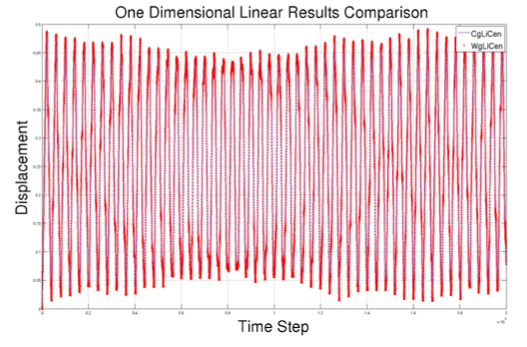
\includegraphics[width=0.8\textwidth]{./pics/result1d2.png}
      	      	\end{tabular}
      	      	\caption{\footnotesize The results comparison between CG only and hybrid WG-CG element for explicit scheme}
      	      \end{figure}
      	      
      	       \begin{figure}[H]
      	       	\centering
      	       	\begin{tabular}{c}
      	       		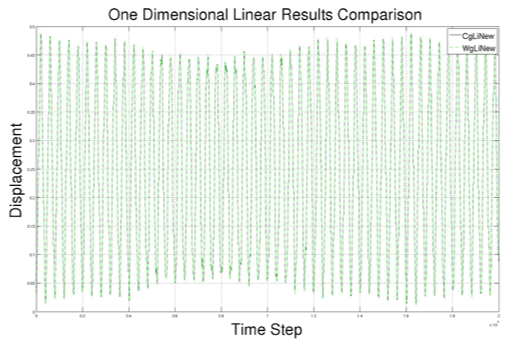
\includegraphics[width=0.8\textwidth]{./pics/result1d3.png}
      	       	\end{tabular}
      	       	\caption{\footnotesize The results comparison between CG only and hybrid WG-CG element for implicit scheme}
      	       \end{figure}
      	       
      	       The above two figures illustrates the comparison of deflections. We compare the solutions between our hybrid WG-CG element and classic CG element. In both implicit and explicit time marching scheme, the average difference between two methods is less than $ 10^{-5} $. Based on the results, our hybrid WG-CG solver shows optimal convergence to the established CG solver. The lower error value encouraged us to extend the hybrid element to handle geometric nonlinear problems.
      	       
 \subsection{Geometric nonlinear elasticity equation}
 
 Both the large deflection and body rotation require the nonlinear strain-displacement relation. We test the performance of accuracy and efficiency of hybrid WG-CG element. We continue using the classic CG element solver as the reference and compare our new method to the reliable existing solutions.
 
 By following the linear elastic equation test cases, we load constant force as the boundary condition and compare the solutions between the serial CG solver and parallel implicit hybrid WG-CG solver. We divide the entire computational domain into 20 subdomains. In another word, each subdomain corresponds to an individual hybrid WG-CG element. In each hybrid element, we insert 20 standard CG elements. Each processor handles one hybrid element and the communicates with each other through MPI library. 
 
 The CG solver choose 400 standard linear CG elements to maintain the same resolution. We track the deflection on the right tip of the domain and plot the two sets of solutions in the same figure to compare the difference as following
 
  \begin{figure}[H]
  	\centering
  	\begin{tabular}{c}
  		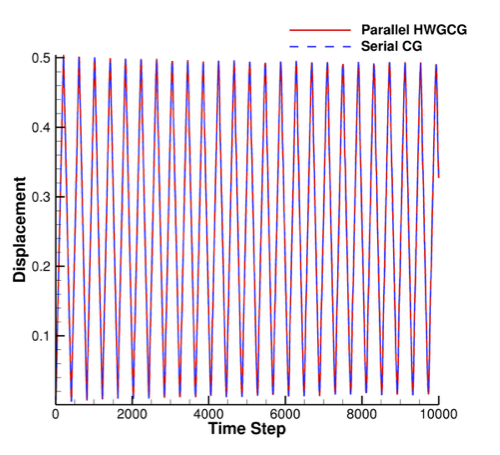
\includegraphics[width=0.8\textwidth]{./pics/result1d4.png}
  	\end{tabular}
  	\caption{\footnotesize The results comparison between CG only and hybrid WG-CG element by using parallel implicit scheme with constant boundary condition}
  \end{figure}
  
  An optimal convergence of the two independent solutions shows an excellent accuracy of the parallel hybrid solver. The average difference is less than $ 10^{-4} $, which is same as the previous linear test.
  
  To verify the the robustness of the new solver, a periodic boundary condition is enforced to substitute the constant variable where $ f = sin (2 \pi t) $. The comparing results is as following chart
  
    \begin{figure}[H]
    	\centering
    	\begin{tabular}{c}
    		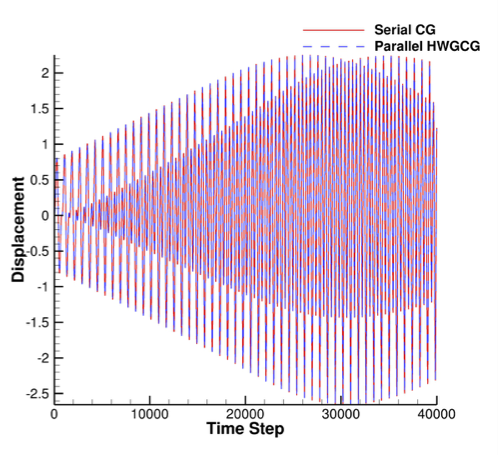
\includegraphics[width=0.8\textwidth]{./pics/result1d5.png}
    	\end{tabular}
    	\caption{\footnotesize The results comparison between CG only and hybrid WG-CG element by using parallel implicit scheme with periodic boundary condition}
    \end{figure}
    
    Analogously, an optimal convergence is also observed from this test case. We have a strong confidence on the accuracy of our nonlinear parallel computing solver. 
    
    After the verification of accuracy and precision, we want to test the performance and parallel computing scalability on high performance clusters. We increase the size of the problem to a higher level, 20 times larger than the original test case, up to 100,000 unknown variables. Meanwhile, we gradually increase the number of processor applied for the problem from 10 to 60. The time using graph is plotted as following
    
  \begin{figure}[H]
  	\centering
  	\begin{tabular}{c}
  		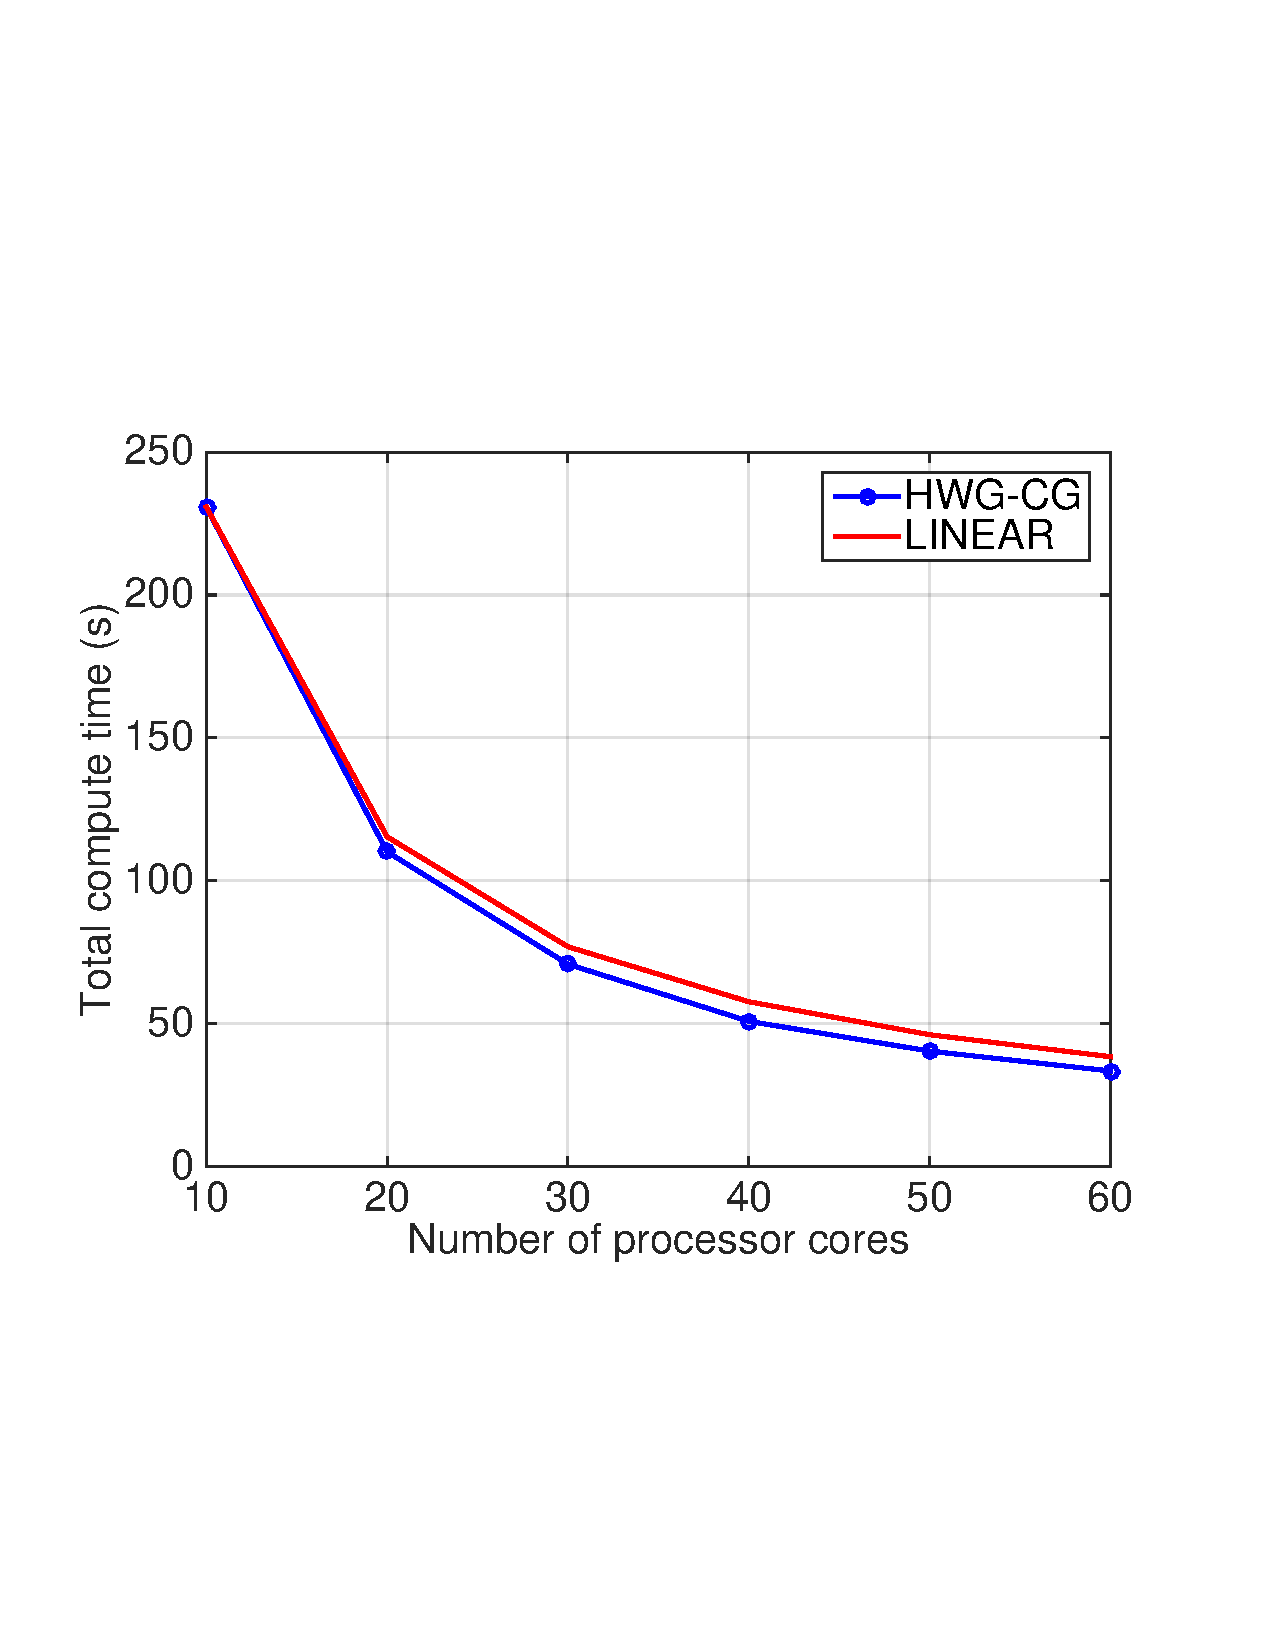
\includegraphics[width=0.7\textwidth]{./pics/lineartime}
  	\end{tabular}
  	\caption{\footnotesize Time decreasing .vs. number of processors increasing}
  \end{figure}
  
  then we also plot the speedup curvature is proportional to the increasing number of processors
   
   \begin{figure}[H]
   	\centering
   	\begin{tabular}{c}
   		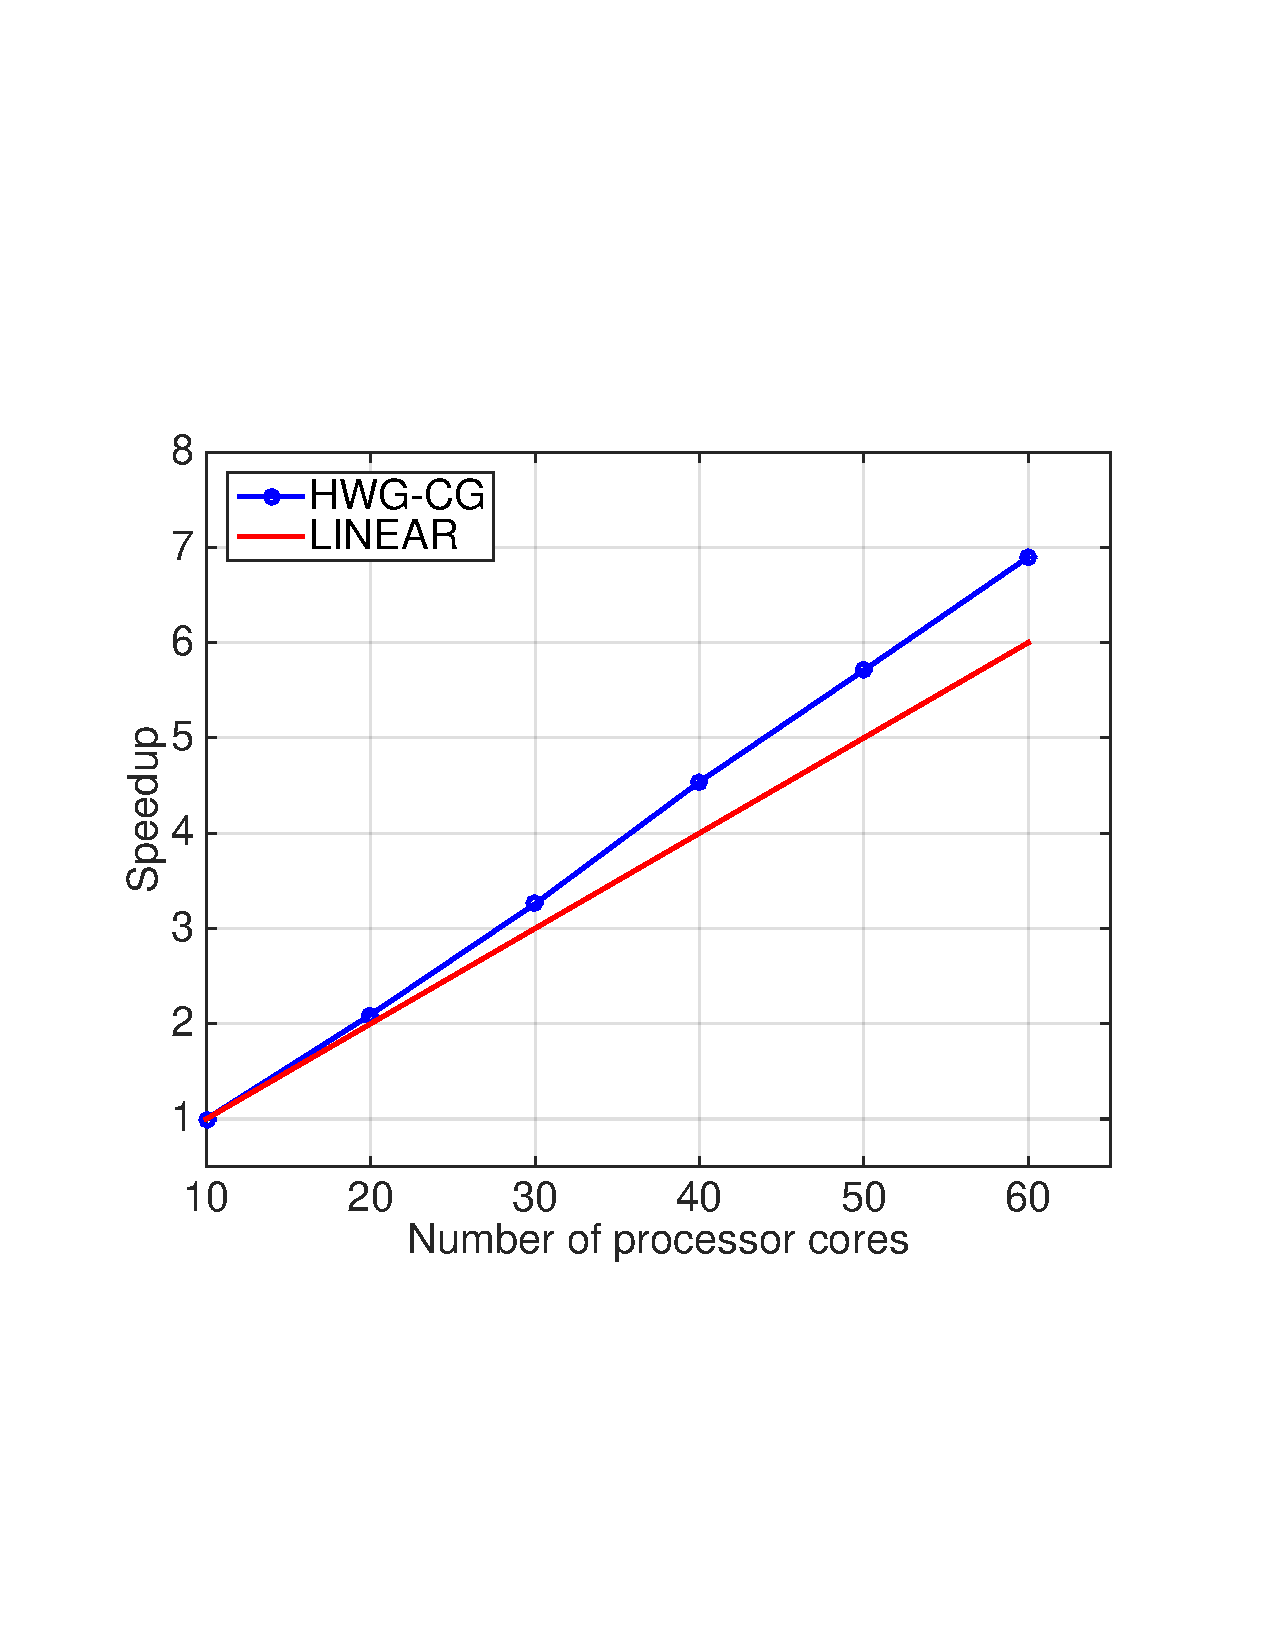
\includegraphics[width=0.7\textwidth]{./pics/linearSp}
   	\end{tabular}
   	\caption{\footnotesize Speedup .vs. number of processors increasing}
   \end{figure}
   
   A superlinear speedup is observed from the above test cases. The reason is that the computational effort to solve local matrices decreases faster than communication overhead. The computational cost for stiffness matrix inverion is $ O(n^{3}) $, where $ n $ is the size of stiffness matrix. Meanwhile, the communication overhead grows linearly with time complexity $ O(n) $.  Overall, the trade-off benefit for domain decomposition is larger than MPI communication which leads to the superlinear results. 
   
   
   		\section{Summary}
   		
   		In summary, we present a newly developed hybrid element combining the weak Galerkin finite element and continuous Galerkin finite element. It inherits the discontinuous feature from WG method and the computational simplicity from CG method. The implementation of hybrid element for parallel computing is through Schur complement method. The second order of accuracy and superlinear speedup are observed for the hybrid element. 
   		
   		We test the hybrid WG-CG element for linear and nonlinear elasticity equations. We implement explicit (Central Difference) and implicit (Newmark-Beta) methods to obtain the results. Comparing with analytical solution and published results, the error is lower than $ 10^{-5} $ for both Dirichlet and Neumann boundary condition.
   		
   		After the one dimensional examples, we present the test cases of the WG method for solving two dimensional problems.We obtain expected order of accuracy. The next step is to implement parallel computing scheme on it. The details of parallel computing for larger problem will be discussed in the next chapter.